\documentclass[12pt,a4paper]{article}
\usepackage[a4paper, margin=0.8in, headheight=14pt]{geometry}
\usepackage{fontspec}
\usepackage{unicode-math}
\setmainfont{TeX Gyre Pagella}
\setmonofont[Scale=0.88]{TeX Gyre Cursor}
\setmathfont{Latin Modern Math}
\usepackage{xcolor}
\usepackage{colortbl}
\usepackage{titlesec}
\usepackage{enumitem}
\usepackage{tabularx}
\usepackage{booktabs}
\usepackage{array}
\usepackage{amsmath}
\usepackage{tikz}
\usetikzlibrary{shapes.geometric, arrows.meta, positioning, calc, fit, decorations.pathreplacing, decorations.pathmorphing, patterns, backgrounds}
\usepackage[american]{circuitikz}
\usepackage{tcolorbox}
\tcbuselibrary{skins, breakable}
\usepackage{etoolbox}
\usepackage{hyperref}
\usepackage{fancyhdr}
\usepackage{graphicx}
\usepackage{microtype}
\hyphenpenalty=10000
\exhyphenpenalty=10000
\sloppy
\usepackage{caption}
\usepackage{setspace}
\usepackage{multirow}
\usepackage{tocloft}
\newcommand{\Q}[1]{\textbf{#1}\par\noindent\ignorespaces}
\definecolor{myred}{RGB}{196,30,58}       % section headings
\definecolor{mydark}{RGB}{30,30,50}       % body text
\definecolor{mygreen}{RGB}{14,120,80}     % definition boxes
\definecolor{myteal}{RGB}{0,130,140}      % formula boxes, diagrams, subsection headings
\definecolor{myamber}{RGB}{180,100,0}     % example boxes
\definecolor{mypurple}{RGB}{100,30,160}   % exam/viva boxes
\definecolor{myblue}{RGB}{25,90,170}      % hyperlinks/diagrams
\definecolor{mygray}{RGB}{246,247,249}    % tikzbox background
\definecolor{mgframe}{RGB}{180,185,200}   % tikzbox border
\definecolor{watermark}{RGB}{145,150,170} % footer watermark
\definecolor{hdrred}{RGB}{250,232,235}
\definecolor{hdrgreen}{RGB}{220,244,233}
\definecolor{hdrteal}{RGB}{220,242,244}
\definecolor{hdramber}{RGB}{253,242,215}
\definecolor{hdrpurple}{RGB}{238,228,255}
\definecolor{hdrblue}{RGB}{235,242,250}
\AfterEndEnvironment{tcolorbox}{\color{mydark}}

\titleformat{\section}{\large\bfseries\color{myred}}{\thesection.}{0.5em}{}[\vspace{1pt}{\color{myred}\rule{\linewidth}{0.8pt}}]
\titleformat{\subsection}{\normalsize\bfseries\color{myteal}}{\thesubsection}{0.5em}{}
\titlespacing*{\section}{0pt}{18pt}{7pt}
\titlespacing*{\subsection}{0pt}{11pt}{4pt}
\setlength{\parindent}{0pt}
\setlength{\parskip}{4pt}
\renewcommand{\cfttoctitlefont}{\large\bfseries\color{myred}}
\renewcommand{\cftaftertoctitle}{\par\noindent{\color{myred}\rule{\linewidth}{0.8pt}}}
\setlength{\cftbeforetoctitleskip}{0pt}
\setlength{\cftaftertoctitleskip}{6pt}
\renewcommand{\cftsecfont}{\normalsize\bfseries\color{mydark}}
\renewcommand{\cftsecpagefont}{\normalsize\bfseries\color{mydark}}
\renewcommand{\cftsecleader}{\cftdotfill{\cftdotsep}}
\setlength{\cftbeforesecskip}{7pt}
\renewcommand{\cftsubsecfont}{\small\color{mydark}}
\renewcommand{\cftsubsecpagefont}{\small\color{mydark}}
\setlength{\cftbeforesubsecskip}{3pt}
\setlength{\cftsubsecindent}{1.4em}
\renewcommand{\cftpartfont}{\normalsize\bfseries\color{myteal}}
\renewcommand{\cftpartpagefont}{\normalsize\bfseries\color{myteal}}
\setlength{\cftbeforepartskip}{14pt}
\renewcommand{\arraystretch}{1.45}
\setlength{\tabcolsep}{6pt}
\arrayrulecolor{mydark}
\newcolumntype{B}[1]{>{\small\bfseries\raggedright\arraybackslash}m{#1}}
\newcolumntype{C}[1]{>{\centering\arraybackslash}m{#1}}
\newcolumntype{Y}{>{\small\raggedright\arraybackslash}X}
\renewcommand{\tabularxcolumn}[1]{m{#1}}
\newcommand{\currmodule}{Module 1}
\pagestyle{fancy}
\fancyhf{}
\fancyhead[L]{\small\color{myred}\textbf{OE-EC804B}\;\color{mydark}--- Microwave Integrated Circuits}
\fancyhead[R]{\small\color{myteal}\textbf{\currmodule\ Notes}}
\fancyfoot[C]{\small\color{mydark}\thepage}
\fancyfoot[R]{\small\color{watermark}\textit{\copyright\ Biraj}}
\renewcommand{\headrulewidth}{0.5pt}
\renewcommand{\footrulewidth}{0.3pt}

\hypersetup{colorlinks=true, linkcolor=myteal, urlcolor=myteal,
  pdfauthor={Biraj Sarkar},
  pdftitle={OE-EC804B --- Combined Notes}}

\tcbset{
  tikzbox/.style={colback=mygray, colframe=mgframe, boxrule=0.6pt, arc=4pt,
    left=8pt, right=8pt, top=6pt, bottom=6pt,
    colbacktitle=mgframe, coltitle=mydark, fonttitle=\small\bfseries},
  defbox/.style={colback=hdrgreen, colframe=mygreen, boxrule=0.8pt, arc=4pt,
    left=9pt, right=9pt, top=6pt, bottom=6pt,
    colbacktitle=mygreen, coltitle=white, fonttitle=\small\bfseries},
  formulabox/.style={colback=hdrteal, colframe=myteal, boxrule=0.8pt, arc=4pt,
    left=9pt, right=9pt, top=7pt, bottom=7pt,
    colbacktitle=myteal, coltitle=white, fonttitle=\small\bfseries},
  examplebox/.style={colback=hdramber, colframe=myamber, boxrule=0.8pt, arc=4pt,
    left=9pt, right=9pt, top=6pt, bottom=6pt,
    colbacktitle=myamber, coltitle=white, fonttitle=\small\bfseries},
  masonbox/.style={colback=hdrpurple, colframe=mypurple, boxrule=0.8pt, arc=4pt,
    left=9pt, right=9pt, top=6pt, bottom=6pt,
    colbacktitle=mypurple, coltitle=white, fonttitle=\small\bfseries},
  exambox/.style={colback=hdrpurple, colframe=mypurple, boxrule=1pt, arc=5pt,
    left=10pt, right=10pt, top=8pt, bottom=8pt,
    colbacktitle=mypurple, coltitle=white, fonttitle=\bfseries,
    title after break={\textbf{Frequently Asked / Viva Questions (contd.)}}}
}
\tcbset{breakable}
\tcbset{coltext=mydark}
\tcbset{after={\color{mydark}}}

\tikzset{
  block/.style={rectangle, draw=myteal, fill=hdrteal, text width=2.4cm, align=center, minimum height=0.95cm, font=\small, rounded corners=3pt, line width=0.7pt},
  redblock/.style={rectangle, draw=myred, fill=hdrred, text width=2.4cm, align=center, minimum height=0.95cm, font=\small, rounded corners=3pt, line width=0.7pt},
  arrow/.style={-Stealth, thick, color=mydark},
  line/.style={thick, color=mydark}
}

\newcommand{\modulestart}[2]{%
  \clearpage
  \renewcommand{\currmodule}{Module #1}%
  \renewcommand{\theHsection}{mod#1.\arabic{section}}%
  \renewcommand{\theHsubsection}{\theHsection.\arabic{subsection}}%
  \renewcommand{\theHsubsubsection}{\theHsubsection.\arabic{subsubsection}}%
  \phantomsection
  \addcontentsline{toc}{part}{Module #1: #2}%
  \setcounter{section}{0}%
  \begin{center}
    \vspace*{1.0cm}
    {\Huge\bfseries\color{myred} Module #1}\\[10pt]
    {\Large\bfseries\color{mydark} #2}\\[10pt]
    {\color{myred}\rule{0.55\linewidth}{1.2pt}}
  \end{center}
  \vspace{14pt}
}
\begin{document}

\thispagestyle{empty}

% ─── Page Border (TikZ Overlay) ────────────────────────────────────────────────
\begin{tikzpicture}[remember picture, overlay]
  % Outer border (fine line in mgframe)
  \draw[color=mgframe, line width=1.5pt] 
    ($(current page.north west) + (0.6in, -0.6in)$) rectangle 
    ($(current page.south east) + (-0.6in, 0.6in)$);
  % Inner border (finer accent line in myred)
  \draw[color=myred, line width=0.8pt] 
    ($(current page.north west) + (0.65in, -0.65in)$) rectangle 
    ($(current page.south east) + (-0.65in, 0.65in)$);
\end{tikzpicture}

\vspace*{1.0cm}
\begin{center}
  {\Huge\bfseries\color{myred} OE-EC804B}\\[10pt]
  {\LARGE\bfseries\color{mydark} Microwave Integrated Circuits}\\[20pt]
  {\color{myred}\rule{0.7\linewidth}{1.5pt}}\\[18pt]
  {\Large\color{myteal}\textbf{Combined Module Notes}}\\[8pt]
  {\large\color{mydark} Modules 1 -- 5}\\[40pt]
  {\normalsize\color{mydark} Semester VIII \quad$\bullet$\quad ECE \quad$\bullet$\quad 3 Credits}\\[12pt]
  {\normalsize\color{mydark} CGEC \;$|$\; B.Tech ECE (2023--27)}
\end{center}
\vspace{1.0cm}
\begin{center}
  \begin{tcolorbox}[colback=mygray, colframe=mgframe, boxrule=0.5pt, arc=3pt, width=0.85\linewidth]
    \centering\small\color{mydark}
    \textbf{Disclaimer / Study Guide Notice:}\\
    These are condensed \textbf{Short Notes} focusing on core theory, key formulas, block/circuit diagrams, and standard viva Q\&As for university exam revision. Exhaustive numerical practice problems and derivation edge cases are not covered. This serves as a quick-revision reference guide for students.
  \end{tcolorbox}
\end{center}
\vfill
\vspace{0.6cm}
\begin{center}
  {\large\bfseries\color{mypurple} Biraj Sarkar}\\[16pt]
  {\footnotesize\color{watermark}\textbf{IN ASSOCIATION WITH}}\\[8pt]
  {\small\bfseries\color{mydark} MAKAUT Wingman \quad$\bullet$\quad MAKAUT Future Minds}\\[12pt]
  {\large\bfseries\color{myteal} Cooch Behar Government Engineering College}
\end{center}
\vfill
\begin{center}{\small\color{watermark}\textit{Exam-Ready Notes}}\end{center}
\clearpage

\hypersetup{linkcolor=mydark}
\tableofcontents
\hypersetup{linkcolor=myteal}
\clearpage

% -- Module 1 -----------------------------------------------------------------
\modulestart{1}{Introduction to MIC and MMIC}

\section{Introduction to MIC and MMIC}

Microwave Integrated Circuits (MICs) operate in the high-frequency spectrum ranging from $300\text{ MHz}$ to $300\text{ GHz}$ (wavelengths $\lambda = 1\text{ m}$ to $1\text{ mm}$). Conventional low-frequency lumped elements (discrete resistors, capacitors, and inductors) fail at microwave frequencies due to parasitic lead inductances and stray capacitances. MIC technology replaces bulky 3D waveguide structures with planar transmission lines printed directly on insulating or semiconductor substrates.

\begin{tcolorbox}[defbox, title={Microwave Integrated Circuit (MIC)}]
  A \textbf{Microwave Integrated Circuit (MIC)} is a high-frequency planar assembly where passive circuit elements (printed microstrip lines, inductors, capacitors, couplers) and active semiconductor devices (diodes, MESFETs, HEMTs, HBTs) are integrated on a common planar substrate.
\end{tcolorbox}

\subsection{Classification: Hybrid MIC (HMIC) vs. Monolithic MIC (MMIC)}

MICs are categorized into two major technological generations:

\begin{enumerate}[leftmargin=*, itemsep=5pt]
  \item \textbf{Hybrid MIC (HMIC):} Passive matching networks and transmission lines are fabricated on a passive dielectric substrate (such as Alumina $\text{Al}_2\text{O}_3$, Quartz, or Sapphire) using thin or thick film deposition. Active semiconductor devices (packaged or unpackaged GaAs/Si FET dies, Schottky/PIN diodes) are individually mounted onto the substrate and connected using gold wire bonds or ribbon bonds.
  \item \textbf{Monolithic MIC (MMIC):} All active semiconductor devices (MESFETs, HEMTs, HBTs), passive matching components (MIM capacitors, thin film resistors, spiral inductors), and planar interconnect transmission lines are grown, etched, and metallized \textbf{simultaneously on a single semiconductor wafer} (such as Gallium Arsenide GaAs, Indium Phosphide InP, or Gallium Nitride GaN).
\end{enumerate}

\par\vspace{6pt}\noindent
\begingroup
\renewcommand{\arraystretch}{1.4}%
\begin{tabularx}{\linewidth}{|>{\raggedright\arraybackslash\bfseries}p{3.2cm}|Y|Y|}
\hline
\textbf{Feature} & \textbf{Hybrid MIC (HMIC)} & \textbf{Monolithic MIC (MMIC)} \\
\hline
Substrate Material & Dielectric (Alumina $\text{Al}_2\text{O}_3$, Quartz, Sapphire, PTFE) & Semi-insulating Semiconductor (GaAs, InP, GaN, SiGe) \\
\hline
Active Device Integration & Discrete semiconductor dies mounted \& wire-bonded individually & Fabricated monolithically directly inside/on the semiconductor wafer \\
\hline
Parasitic Reactance & High due to wire bond inductances ($L_s \approx 0.5 - 2\text{ nH}$) & Negligible; planar interconnects eliminate bond wire inductances \\
\hline
Frequency Range & Typically $< 20\text{ GHz}$ due to bond wire parasitics & Millimeter-wave up to $300\text{ GHz}$ and THz frequencies \\
\hline
Production Volume & Ideal for prototype development and low-volume production & Highly economical for mass batch production ($10^4 - 10^7$ units) \\
\hline
Unit Cost & Low initial mask cost; high unit assembly labor cost & High initial mask/NRE cost; extremely low per-chip unit cost \\
\hline
Post-Fabrication Tuning & Trimming of capacitors/resistors possible post-fabrication & No post-fabrication tuning possible; design must be 100\% accurate \\
\hline
Thermal Dissipation & Excellent thermal transfer through thick ceramic substrates & Moderate to poor; requires thermal via holes through wafer \\
\hline
\end{tabularx}
\endgroup

\subsection{Advantages of MICs over Discrete \& Waveguide Circuits}
\begin{itemize}[leftmargin=*, itemsep=4pt]
  \item \textbf{Miniaturization \& Weight Reduction:} Planar integration reduces volume and weight by over $90\%$ compared to metallic waveguides.
  \item \textbf{High Reliability \& Reproducibility:} Batch photolithography eliminates mechanical assembly variations and hand-soldered joints.
  \item \textbf{Broadband Performance:} Short planar interconnects minimize parasitic leads, extending operating bandwidths to multi-octave ranges.
  \item \textbf{Multifunctional Systems-on-Chip (SoC):} Enables complete transmit/receive (T/R) radar modules on a single die.
\end{itemize}

% ===============================================================================
% 2. MMIC FABRICATION TECHNIQUES AND MATERIALS
% ===============================================================================
\section{MMIC Fabrication Techniques and Materials}

\subsection{Substrate Materials for MMICs}
The choice of substrate dictates electrical attenuation, substrate power loss, high-frequency cutoff, and power dissipation capabilities.

\begin{tcolorbox}[masonbox, title={Substrate Requirements for MMICs}]
  An ideal MMIC substrate must exhibit:
  \begin{enumerate}[leftmargin=*, noitemsep]
    \item High electrical resistivity ($\rho > 10^7\text{ }\Omega\cdot\text{cm}$) to minimize RF substrate conduction losses.
    \item Low dielectric loss tangent ($\tan\delta < 0.001$) for minimal wave attenuation.
    \item High thermal conductivity ($K$) to dissipate heat from high-power active devices.
    \item High electron mobility ($\mu_e$) to enable high-speed transistor switching.
  \end{enumerate}
\end{tcolorbox}

\par\vspace{6pt}\noindent
\begingroup
\renewcommand{\arraystretch}{1.4}%
\begin{tabularx}{\linewidth}{|>{\raggedright\arraybackslash\bfseries}p{2.5cm}|>{\centering\arraybackslash}X|>{\centering\arraybackslash}X|>{\centering\arraybackslash}X|>{\raggedright\arraybackslash}X|}
\hline
\textbf{Substrate} & \textbf{Dielectric Constant ($\varepsilon_r$)} & \textbf{Loss Tangent ($\tan\delta$)} & \textbf{Thermal Cond. ($W/cm\cdot K$)} & \textbf{Key Properties \& Applications} \\
\hline
Gallium Arsenide (GaAs) & $12.9$ & $0.0006$ & $0.46$ & Standard workhorse for MMICs up to $100\text{ GHz}$; high mobility ($\mu_e = 8500\text{ cm}^2/\text{V}\cdot\text{s}$). \\
\hline
Indium Phosphide (InP) & $12.4$ & $0.0010$ & $0.68$ & Sub-millimeter wave and THz MMICs ($>100\text{ GHz}$); ultra-high peak electron velocity. \\
\hline
Gallium Nitride (GaN) & $8.9$ & $0.0005$ & $1.30$ & High-power microwave amplifiers; high breakdown field ($3\text{ MV/cm}$). \\
\hline
Silicon (Si / High-Res) & $11.7$ & $0.0050$ & $1.45$ & RF-CMOS and SiGe HBT integration; cheap mass production up to $60\text{ GHz}$. \\
\hline
Alumina ($\text{Al}_2\text{O}_3$) & $9.8$ & $0.0001$ & $0.30$ & Standard substrate for Hybrid MICs; excellent dielectric stability. \\
\hline
\end{tabularx}
\endgroup

\subsection{Thin Film Technology (Film Thickness \texorpdfstring{$< 5\text{ }\mu\text{m}$}{< 5 um})}
Thin film technology is used in all high-frequency MMICs and precision Hybrid MICs.

\begin{itemize}[leftmargin=*, itemsep=4pt]
  \item \textbf{Deposition Methods:}
    \begin{itemize}[leftmargin=*, noitemsep]
      \item \textit{Vacuum Evaporation:} Thermal or electron-beam heating vaporizes metal atoms in high vacuum ($10^{-6}\text{ Torr}$).
      \item \textit{RF Sputtering:} Argon ions bombard a target material, knocking off atoms that deposit uniformly onto the substrate.
      \item \textit{Electroplating:} Electro-chemical growth used to thicken conductor traces to several skin depths ($2-5\text{ }\mu\text{m}$ of Gold Au).
    \end{itemize}
  \item \textbf{Passive Component Fabrication:}
    \begin{itemize}[leftmargin=*, noitemsep]
      \item \textit{Thin Film Resistors:} Tantalum Nitride ($\text{TaN}$) or Nickel Chromium ($\text{NiCr}$) providing sheet resistivities of $10 - 100\text{ }\Omega/\text{sq}$.
      \item \textit{Metal-Insulator-Metal (MIM) Capacitors:} Top and bottom Gold plates separated by a thin dielectric film of Silicon Nitride ($\text{Si}_3\text{N}_4$, $\varepsilon_r=7.5$) or Silicon Dioxide ($\text{SiO}_2$, $\varepsilon_r=3.9$).
    \end{itemize}
\end{itemize}

\subsection{Thick Film Technology (Film Thickness \texorpdfstring{$10 - 50\text{ }\mu\text{m}$}{10 - 50 um})}
Used primarily for low-frequency, high-power Hybrid MICs below $10\text{ GHz}$.
\begin{itemize}[leftmargin=*, itemsep=3pt]
  \item Deposited via \textbf{Screen Printing} of conductive or resistive pastes through fine stainless-steel mesh screens onto ceramic substrates.
  \item Fired in high-temperature belt furnaces at $850^\circ\text{C}$ to sinter metal particles.
  \item Minimum resolution is limited to $>75\text{ }\mu\text{m}$ line widths.
\end{itemize}

\begin{tcolorbox}[tikzbox, title={Cross-Sectional Structure of Thin-Film MIM Capacitor and Microstrip Line on GaAs}]
\centering
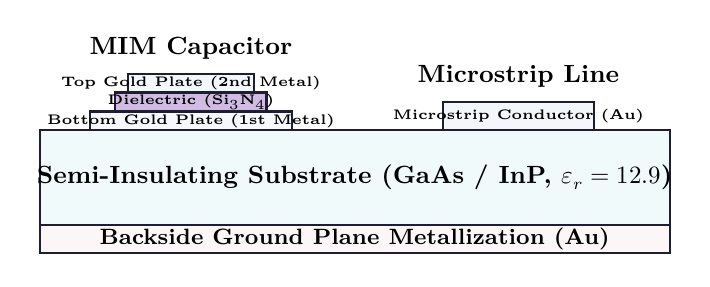
\begin{tikzpicture}[x=1.6cm, y=1.2cm]
  % Substrate
  \draw[line, fill=hdrteal!40] (0,0) rectangle (5.0,1.0);
  \node at (2.5,0.5) {\small\textbf{Semi-Insulating Substrate (GaAs / InP, $\varepsilon_r = 12.9$)}};
  
  % Ground Plane
  \draw[line, fill=hdrred!40] (0,-0.3) rectangle (5.0,0);
  \node at (2.5,-0.15) {\footnotesize\textbf{Backside Ground Plane Metallization (Au)}};
  
  % MIM Capacitor - Bottom Plate
  \draw[line, fill=hdrblue!50] (0.4,1) rectangle (2.0,1.2);
  \node at (1.2,1.1) {\tiny\textbf{Bottom Gold Plate (1st Metal)}};
  
  % MIM Dielectric
  \draw[line, fill=mypurple!30] (0.6,1.2) rectangle (1.8,1.4);
  \node at (1.2,1.3) {\tiny\textbf{Dielectric ($\text{Si}_3\text{N}_4$)}};
  
  % MIM Top Plate
  \draw[line, fill=hdrblue!60] (0.7,1.4) rectangle (1.7,1.6);
  \node at (1.2,1.5) {\tiny\textbf{Top Gold Plate (2nd Metal)}};
  
  % Microstrip Line
  \draw[line, fill=hdrblue!60] (3.2,1) rectangle (4.4,1.3);
  \node at (3.8,1.15) {\tiny\textbf{Microstrip Conductor (Au)}};
  
  % Labels
  \node[anchor=south] at (1.2,1.65) {\small\textbf{MIM Capacitor}};
  \node[anchor=south] at (3.8,1.35) {\small\textbf{Microstrip Line}};
\end{tikzpicture}
\end{tcolorbox}

\begin{tcolorbox}[examplebox, title={MIM Capacitor Calculation}]
  \textbf{Problem:} Calculate the required area of a Silicon Nitride ($\text{Si}_3\text{N}_4$, $\varepsilon_r = 7.5$) MIM capacitor to achieve a capacitance of $C = 10\text{ pF}$ if the dielectric thickness is $d = 2000\text{ \AA}$ ($200\text{ nm}$).
  \tcblower
  \textbf{Solution:}
  Using the parallel-plate capacitance formula:
  \begin{equation}
    C = \frac{\varepsilon_0 \varepsilon_r A}{d} \implies A = \frac{C \cdot d}{\varepsilon_0 \varepsilon_r}
  \end{equation}
  Given: $C = 10 \times 10^{-12}\text{ F}$, $d = 200 \times 10^{-9}\text{ m}$, $\varepsilon_0 = 8.854 \times 10^{-12}\text{ F/m}$, $\varepsilon_r = 7.5$.
  \begin{equation}
    \begin{aligned}
      A &= \frac{(10 \times 10^{-12}) \times (200 \times 10^{-9})}{(8.854 \times 10^{-12}) \times 7.5} \\
      &= \frac{2 \times 10^{-18}}{6.6405 \times 10^{-11}} = 3.0118 \times 10^{-8}\text{ m}^2 = 0.0301\text{ mm}^2
    \end{aligned}
  \end{equation}
  For a square capacitor plate of length $L$:
  \begin{equation}
    L = \sqrt{A} = \sqrt{0.0301\text{ mm}^2} \approx 0.1735\text{ mm} = 173.5\text{ }\mu\text{m}
  \end{equation}
\end{tcolorbox}

% ===============================================================================
% 3. ENCAPSULATION AND MOUNTING OF ACTIVE DEVICES
% ===============================================================================
\section{Encapsulation and Mounting of Active Devices}

\subsection{Active Device Mounting Techniques}
In Hybrid MICs, discrete active semiconductor chips (diodes, MESFETs, HBTs) must be attached to the substrate and interconnected to microstrip lines. Three primary mounting techniques are utilized:

\begin{enumerate}[leftmargin=*, itemsep=5pt]
  \item \textbf{Wire Bonding (Thermosonic / Ultrasonic):}
    \begin{itemize}[leftmargin=*, noitemsep]
      \item Fine Gold ($\text{Au}$) wires ($17.5 - 25\text{ }\mu\text{m}$ diameter) connect die pads to substrate traces.
      \item \textit{Drawback:} Introduces parasitic series inductance $L_s \approx 1\text{ nH/mm}$. At $20\text{ GHz}$, a $1\text{ mm}$ wire bond introduces an inductive reactance $X_L = 2\pi f L_s = 2\pi (20 \times 10^9) (10^{-9}) = 125.66\text{ }\Omega$, destroying impedance matching!
    \end{itemize}
  \item \textbf{Flip-Chip Bonding:}
    \begin{itemize}[leftmargin=*, noitemsep]
      \item The semiconductor die is inverted face-down and attached directly to substrate pads via solder bumps or gold pillars ($20 - 50\text{ }\mu\text{m}$ height).
      \item Reduces parasitic series inductance by over $95\%$ ($L_s < 0.05\text{ nH}$), enabling performance up to $100\text{ GHz}$.
    \end{itemize}
  \item \textbf{Tape Automated Bonding (TAB):}
    \begin{itemize}[leftmargin=*, noitemsep]
      \item Patterned copper foil leads on a flexible polyimide film are gang-bonded simultaneously to die pads.
    \end{itemize}
\end{enumerate}

\subsection{Encapsulation and Package Requirements}
Packaging protects delicate GaAs/InP devices from environmental humidity, oxidation, and mechanical stress while providing a low-reflection $50\text{ }\Omega$ RF path.

\begin{tcolorbox}[defbox, title={Hermetic Packaging}]
  \textbf{Hermetic Packaging} encloses MIC/MMIC circuits inside glass-sealed ceramic or laser-welded metal housings filled with dry nitrogen, preventing moisture ingress and long-term performance degradation.
\end{tcolorbox}

% ===============================================================================
% QUICK REVISION PAGE
% ===============================================================================
\newpage
\begin{center}
  {\large\bfseries\color{myred} Quick Revision --- Module 1}\\[3pt]
  {\small\color{mydark} Introduction to MIC \& MMIC $|$ OE-EC804B}
\end{center}
\noindent{\color{myred}\rule{\linewidth}{1.2pt}}
\vspace{4pt}

\begin{tcolorbox}[formulabox, title={\textbf{Key Concepts and Metrics at a Glance}}]
\renewcommand{\arraystretch}{1.35}
\begin{tabularx}{\linewidth}{>{\raggedright\arraybackslash\bfseries}p{4.5cm} X}
Hybrid MIC (HMIC) & Passives on dielectric substrate ($\text{Al}_2\text{O}_3$); discrete active dies wire-bonded. \\[4pt]
Monolithic MIC (MMIC) & Passives, active devices, and lines fabricated monolithically on single GaAs/InP wafer. \\[4pt]
Substrate Materials & GaAs ($\varepsilon_r=12.9, \mu_e=8500$), InP ($\varepsilon_r=12.4$), GaN ($\varepsilon_r=8.9, 3\text{ MV/cm}$). \\[4pt]
MIM Capacitance & $C = \frac{\varepsilon_0 \varepsilon_r A}{d}$ \quad ($\text{Si}_3\text{N}_4$ dielectric, $\varepsilon_r = 7.5$). \\[4pt]
Wire Bond Parasitic & $L_s \approx 1\text{ nH/mm} \implies X_L = 2\pi f L_s$; mitigated by Flip-Chip bonding ($<0.05\text{ nH}$). \\
\end{tabularx}
\end{tcolorbox}

\begin{tcolorbox}[defbox, title={\textbf{One-Line Definitions}}]
  \begin{itemize}[leftmargin=*, noitemsep]
    \item \textbf{MMIC:} An integrated circuit containing all active and passive microwave components on a single semiconductor chip.
    \item \textbf{MIM Capacitor:} Metal-Insulator-Metal thin film capacitor providing high capacitance density in MMICs.
    \item \textbf{Loss Tangent ($\tan\delta$):} Ratio of imaginary to real permittivity ($\varepsilon''/\varepsilon'$) measuring dielectric RF dissipation.
    \item \textbf{Flip-Chip Bonding:} Surface-mount method bonding an inverted chip face-down via solder bumps, eliminating wire bond inductance.
  \end{itemize}
\end{tcolorbox}

\begin{tcolorbox}[exambox, title={\textbf{Frequently Asked / Viva Questions}}]
  \begin{enumerate}[topsep=0pt, label=\textbf{Q\arabic*.}, itemsep=5pt]
    \item \Q{Compare Hybrid MICs and Monolithic MICs.}
    HMICs use separate dielectric substrates with individually mounted active chips. MMICs fabricate all active and passive components simultaneously on a single semiconductor substrate (GaAs/InP).

    \item \Q{Why is GaAs preferred over Silicon for MMICs?}
    GaAs is a direct bandgap semiconductor with semi-insulating resistivity ($\rho > 10^7\text{ }\Omega\cdot\text{cm}$) and higher electron mobility ($\mu_e \approx 8500\text{ cm}^2/\text{V}\cdot\text{s}$ vs $1400$ for Si), providing low RF substrate losses.

    \item \Q{What are the advantages of MMICs over discrete microwave circuits?}
    Small size, low weight, high reliability, high reproducibility, elimination of wire bond parasitics, and low mass-production cost.

    \item \Q{Explain Thin Film technology in MIC fabrication.}
    Thin film technology deposits metal and dielectric films ($<5\text{ }\mu\text{m}$) via sputtering or evaporation, using photolithography to achieve high-precision line widths down to sub-micron scales.

    \item \Q{What materials are used for thin film resistors and capacitors?}
    Resistors use Tantalum Nitride ($\text{TaN}$) or Nickel Chromium ($\text{NiCr}$). Capacitors use Metal-Insulator-Metal (MIM) with $\text{Si}_3\text{N}_4$ or $\text{SiO}_2$ dielectrics.

    \item \Q{What is the main electrical drawback of wire bonding at microwave frequencies?}
    Wire bonds introduce parasitic series inductance ($L_s \approx 1\text{ nH/mm}$), causing significant impedance mismatches above $12\text{ GHz}$.

    \item \Q{How does Flip-Chip bonding overcome wire bond parasitics?}
    Flip-Chip bonding mounts the chip face-down directly onto substrate pads using short solder bumps, reducing parasitic inductance by over $90\%$.

    \item \Q{Why is high thermal conductivity critical for MMIC substrate materials?}
    High-power active devices generate significant heat in a small area; high thermal conductivity prevents thermal breakdown and maintains transistor gain.

    \item \Q{Define loss tangent ($\tan\delta$) and its significance in MICs.}
    Loss tangent $\tan\delta = \epsilon'' / \epsilon'$ quantifies dielectric power loss; lower $\tan\delta$ minimizes attenuation in planar transmission lines.

    \item \Q{What is Hermetic Sealing and why is it necessary for MMICs?}
    Hermetic sealing provides an airtight ceramic/metal package protecting unpassivated GaAs active devices from moisture and atmospheric degradation.
  \end{enumerate}
\end{tcolorbox}


% -- Module 2 -----------------------------------------------------------------
\modulestart{2}{Stripline and Microstrip Line Fundamentals}

\section{Stripline and Microstrip Line Fundamentals}

Planar transmission lines form the foundational interconnections and resonant components in MIC design.

\subsection{Stripline Geometry and Pure TEM Propagation}
A \textbf{Stripline} consists of a flat strip conductor of width $W$ and thickness $t$ centered symmetrically inside a dielectric substrate of thickness $b$, bounded above and below by two parallel conducting ground planes.

\begin{tcolorbox}[defbox, title={Stripline Pure TEM Propagation}]
  Because the strip conductor is completely embedded inside a single, homogeneous dielectric medium ($\varepsilon_r$), the wave phase velocity is uniform throughout the cross-section. Stripline supports a \textbf{pure Transverse Electromagnetic (TEM) mode} with zero longitudinal electric ($E_z = 0$) or magnetic ($H_z = 0$) field components.
\end{tcolorbox}

\subsection{Microstrip Line Geometry and Quasi-TEM Mode}
A \textbf{Microstrip Line} consists of a strip conductor of width $W$ and thickness $t$ printed on top of a dielectric substrate of thickness $h$, backed by a single ground plane on the bottom.

\begin{tcolorbox}[masonbox, title={Quasi-TEM Mode in Microstrip}]
  Because the top surface of a microstrip line is open to air ($\varepsilon_r = 1$) while the lower region consists of dielectric ($\varepsilon_r > 1$), the electromagnetic field spans two different dielectric media. The phase velocity in air ($c$) differs from that in the substrate ($c/\sqrt{\varepsilon_r}$). Pure TEM propagation cannot be supported; the fundamental mode is an inhomogeneous \textbf{Quasi-TEM mode} with tiny longitudinal field components ($E_z, H_z \ne 0$).
\end{tcolorbox}

\begin{tcolorbox}[tikzbox, title={Cross-Sectional Geometries and Field Distribution: Stripline vs. Microstrip}]
\centering
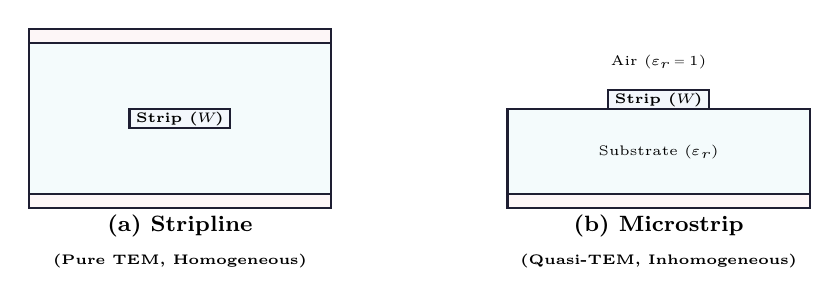
\begin{tikzpicture}[x=1.6cm, y=1.2cm]
  % Stripline Diagram
  \draw[line, fill=hdrteal!30] (0,0) rectangle (2.4,1.6);
  \draw[line, fill=hdrred!40] (0,1.6) rectangle (2.4,1.75); % Top Ground
  \draw[line, fill=hdrred!40] (0,-0.15) rectangle (2.4,0);  % Bottom Ground
  \draw[line, fill=hdrblue!60] (0.8,0.7) rectangle (1.6,0.9); % Center strip
  \node at (1.2,0.8) {\tiny\textbf{Strip ($W$)}};
  \node[align=center] at (1.2,-0.5) {\footnotesize\textbf{(a) Stripline}\\\tiny\textbf{(Pure TEM, Homogeneous)}};
  
  % Microstrip Diagram
  \draw[line, fill=hdrteal!30] (3.8,0) rectangle (6.2,0.9);
  \draw[line, fill=hdrred!40] (3.8,-0.15) rectangle (6.2,0);  % Ground
  \draw[line, fill=hdrblue!60] (4.6,0.9) rectangle (5.4,1.1); % Top strip
  \node at (5.0,1.0) {\tiny\textbf{Strip ($W$)}};
  \node at (5.0,1.4) {\tiny Air ($\varepsilon_r=1$)};
  \node at (5.0,0.45) {\tiny Substrate ($\varepsilon_r$)};
  \node[align=center] at (5.0,-0.5) {\footnotesize\textbf{(b) Microstrip}\\\tiny\textbf{(Quasi-TEM, Inhomogeneous)}};
\end{tikzpicture}
\end{tcolorbox}

% ===============================================================================
% 2. EFFECTIVE DIELECTRIC CONSTANT & IMPEDANCE ANALYSIS
% ===============================================================================
\section{Effective Dielectric Constant (\texorpdfstring{$\varepsilon_{eff}$}{epsilon\_eff}) and Analysis}

\subsection{Concept of Effective Dielectric Constant (\texorpdfstring{$\varepsilon_{eff}$}{epsilon\_eff})}
To simplify the analysis of inhomogeneous microstrip lines, the air-dielectric boundary is replaced by a fictitious homogeneous dielectric medium extending throughout space, characterized by an \textbf{Effective Dielectric Constant ($\varepsilon_{eff}$)}.

\begin{tcolorbox}[formulabox, title={Effective Dielectric Constant ($\varepsilon_{eff}$) Formula}]
  The effective dielectric constant is bounded by $1 < \varepsilon_{eff} < \varepsilon_r$ and is calculated using Schneider's closed-form expression:
  \begin{equation}
    \varepsilon_{eff} = \frac{\varepsilon_r + 1}{2} + \frac{\varepsilon_r - 1}{2} \left[ 1 + 12\frac{h}{W} \right]^{-1/2}
  \end{equation}
  where $W$ is the microstrip width and $h$ is the substrate thickness.
\end{tcolorbox}

\subsection{Guided Wavelength and Phase Velocity}
The phase velocity $v_p$ and guided wavelength $\lambda_g$ in microstrip are given by:
\begin{equation}
  v_p = \frac{c}{\sqrt{\varepsilon_{eff}}} \quad ; \quad \lambda_g = \frac{v_p}{f} = \frac{\lambda_0}{\sqrt{\varepsilon_{eff}}}
\end{equation}

\subsection{Microstrip Characteristic Impedance (\texorpdfstring{$Z_0$}{Z0}) Analysis \& Synthesis}

\begin{enumerate}[leftmargin=*, itemsep=5pt]
  \item \textbf{Analysis Formulas (Given $W/h$ and $\varepsilon_r$, find $Z_0$):}
    \begin{itemize}[leftmargin=*, itemsep=3pt]
      \item For Narrow Strips ($W/h \le 1$):
        \begin{equation}
          Z_0 = \frac{60}{\sqrt{\varepsilon_{eff}}} \ln\left[ 8\frac{h}{W} + 0.25\frac{W}{h} \right]
        \end{equation}
      \item For Wide Strips ($W/h \ge 1$):
        \begin{equation}
          Z_0 = \frac{120\pi}{\sqrt{\varepsilon_{eff}} \left[ \frac{W}{h} + 1.393 + 0.667 \ln\left( \frac{W}{h} + 1.444 \right) \right]}
        \end{equation}
    \end{itemize}

  \item \textbf{Synthesis Formulas (Given target $Z_0$ and $\varepsilon_r$, find required $W/h$):}
    \begin{itemize}[leftmargin=*, itemsep=3pt]
      \item For $W/h < 2$:
        \begin{equation}
          \frac{W}{h} = \frac{8 e^A}{e^{2A} - 2} \quad \text{where } A = \frac{Z_0}{60} \sqrt{\frac{\varepsilon_r+1}{2}} + \frac{\varepsilon_r-1}{\varepsilon_r+1} \left( 0.23 + \frac{0.11}{\varepsilon_r} \right)
        \end{equation}
      \item For $W/h > 2$:
        \begin{equation}
          \frac{W}{h} = \frac{2}{\pi} \left[ B - 1 - \ln(2B-1) + \frac{\varepsilon_r-1}{2\varepsilon_r} \left( \ln(B-1) + 0.39 - \frac{0.61}{\varepsilon_r} \right) \right]
        \end{equation}
        where $B = \frac{377\pi}{2 Z_0 \sqrt{\varepsilon_r}}$.
    \end{itemize}
\end{enumerate}

\subsection{Stripline Characteristic Impedance Formula}
For a symmetrical stripline with ground plane spacing $b$ and effective strip width $W_e$:
\begin{equation}
  Z_{0,\text{strip}} = \frac{30\pi}{\sqrt{\varepsilon_r}} \frac{b}{W_e + 0.441b} \quad \text{where } W_e = W \text{ for } t/b \to 0
\end{equation}

\begin{tcolorbox}[examplebox, title={Worked Numerical: Microstrip Design \& Wavelength Calculation}]
  \textbf{Problem:} A microstrip line is printed on an Alumina substrate ($\varepsilon_r = 9.8$, $h = 0.635\text{ mm}$). If the width-to-height ratio is $W/h = 1.0$, calculate:
  \begin{enumerate}[label=(\alph*), noitemsep]
    \item The effective dielectric constant $\varepsilon_{eff}$.
    \item The characteristic impedance $Z_0$.
    \item The guided wavelength $\lambda_g$ at $10\text{ GHz}$.
  \end{enumerate}
  \tcblower
  \textbf{Solution:}
  \begin{enumerate}[label=(\alph*), itemsep=4pt]
    \item Calculate $\varepsilon_{eff}$ using $W/h = 1.0$:
      \begin{equation}
        \begin{aligned}
          \varepsilon_{eff} &= \frac{9.8 + 1}{2} + \frac{9.8 - 1}{2} \left[ 1 + 12(1) \right]^{-1/2} \\
          &= 5.4 + 4.4 \left[ 13 \right]^{-1/2} = 5.4 + \frac{4.4}{3.6055} \\
          &= 5.4 + 1.2203 = 6.6203
        \end{aligned}
      \end{equation}
    \item Since $W/h = 1.0 \le 1$, use the narrow strip formula for $Z_0$:
      \begin{equation}
        \begin{aligned}
          Z_0 &= \frac{60}{\sqrt{6.6203}} \ln\left[ 8(1) + 0.25(1) \right] \\
          &= \frac{60}{2.573} \ln(8.25) = 23.319 \times 2.1102 \\
          &= 49.21\text{ }\Omega \approx 50\text{ }\Omega
        \end{aligned}
      \end{equation}
    \item Free-space wavelength $\lambda_0 = \frac{c}{f} = \frac{3 \times 10^8\text{ m/s}}{10 \times 10^9\text{ Hz}} = 30\text{ mm}$.
      \begin{equation}
        \lambda_g = \frac{\lambda_0}{\sqrt{\varepsilon_{eff}}} = \frac{30\text{ mm}}{\sqrt{6.6203}} = \frac{30}{2.573} = 11.66\text{ mm}
      \end{equation}
  \end{enumerate}
\end{tcolorbox}

% ===============================================================================
% 3. LOSSES, DISPERSION, AND DISCONTINUITIES
% ===============================================================================
\section{Losses, Dispersion, and Discontinuities in Microstrip}

\subsection{Microstrip Attenuation \& Loss Mechanisms}
Total attenuation constant $\alpha_{total} = \alpha_c + \alpha_d + \alpha_r$ ($\text{Np/m}$ or $\text{dB/m}$):

\begin{itemize}[leftmargin=*, itemsep=4pt]
  \item \textbf{Conductor Loss ($\alpha_c$):} Skin effect causes current to crowd within skin depth $\delta = \sqrt{\frac{1}{\pi f \mu \sigma}}$ along lower surface edges:
    \begin{equation}
      \alpha_c \approx \frac{8.686 R_s}{Z_0 W} \text{ dB/m} \quad \text{where } R_s = \sqrt{\frac{\pi f \mu}{\sigma}} \text{ (Surface Resistance)}
    \end{equation}
  \item \textbf{Dielectric Loss ($\alpha_d$):} Caused by substrate dipole relaxation loss:
    \begin{equation}
      \alpha_d = 27.3 \frac{\varepsilon_r}{\sqrt{\varepsilon_{eff}}} \frac{\varepsilon_{eff}-1}{\varepsilon_r-1} \frac{\tan\delta}{\lambda_0} \quad \text{dB/m}
    \end{equation}
  \item \textbf{Radiation Loss ($\alpha_r$):} At high frequencies, microstrip open boundaries act as long slot radiators emitting RF energy into space.
\end{itemize}

\subsection{Microstrip Discontinuities}
Physical transitions in microstrip layouts alter local electric and magnetic field distributions, generating parasitic reactances.

\par\vspace{6pt}\noindent
\begingroup
\renewcommand{\arraystretch}{1.4}%
\begin{tabularx}{\linewidth}{|>{\raggedright\arraybackslash\bfseries}p{3.2cm}|Y|Y|}
\hline
\textbf{Discontinuity Type} & \textbf{Physical Origin} & \textbf{Equivalent Circuit Model \& Mitigation} \\
\hline
Open-End Line & Fringing electric fields extend past strip termination into air & Shunt end capacitance $C_{oc}$, equivalent to extra length $\Delta l = 0.412 h \frac{\varepsilon_{eff}+0.3}{\varepsilon_{eff}-0.258} \frac{W/h+0.264}{W/h+0.8}$. \\
\hline
Step-Change in Width & Sudden width transition $W_1 \to W_2$ disrupts current distribution & Series inductance $L_s$ and shunt capacitance $C_s$. \\
\hline
Right-Angle Bend ($90^\circ$) & Current crowding at inner corner; excess charge at outer corner & Series inductance $L_b$ and shunt capacitance $C_b$. Mitigated by $45^\circ$ Mitred Bend ($M = 52 + 65 e^{-1.35 W/h}\%$ metal removal). \\
\hline
T-Junction / Cross & Junction of orthogonal microstrip branches & Equivalent $T$-network of series inductances and shunt capacitance. \\
\hline
\end{tabularx}
\endgroup

% ===============================================================================
% QUICK REVISION PAGE
% ===============================================================================
\newpage
\begin{center}
  {\large\bfseries\color{myred} Quick Revision --- Module 2}\\[3pt]
  {\small\color{mydark} Planar Transmission Lines-I (Stripline \& Microstrip) $|$ OE-EC804B}
\end{center}
\noindent{\color{myred}\rule{\linewidth}{1.2pt}}
\vspace{4pt}

\begin{tcolorbox}[formulabox, title={\textbf{Key Concepts and Metrics at a Glance}}]
\renewcommand{\arraystretch}{1.35}
\begin{tabularx}{\linewidth}{>{\raggedright\arraybackslash\bfseries}p{4.5cm} X}
Effective Dielectric $\varepsilon_{eff}$ & $\varepsilon_{eff} = \frac{\varepsilon_r+1}{2} + \frac{\varepsilon_r-1}{2} \left[1 + 12\frac{h}{W}\right]^{-1/2} \quad (1 < \varepsilon_{eff} < \varepsilon_r)$ \\[4pt]
Phase Velocity \& Wavelength & $v_p = \frac{c}{\sqrt{\varepsilon_{eff}}} \quad ; \quad \lambda_g = \frac{\lambda_0}{\sqrt{\varepsilon_{eff}}}$ \\[4pt]
Stripline Propagation & Pure TEM mode ($E_z=0, H_z=0$) due to symmetrical homogeneous dielectric. \\[4pt]
Microstrip Propagation & Inhomogeneous Quasi-TEM mode ($E_z, H_z \ne 0$) due to air-substrate boundary. \\[4pt]
Mitred Bend Optimal Cut & $M = \frac{x}{d\sqrt{2}} \times 100\% = 52 + 65 e^{-1.35 W/h}\%$ removes $90^\circ$ corner capacitance. \\
\end{tabularx}
\end{tcolorbox}

\begin{tcolorbox}[defbox, title={\textbf{One-Line Definitions}}]
  \begin{itemize}[leftmargin=*, noitemsep]
    \item \textbf{Quasi-TEM Mode:} Hybrid electromagnetic wave in non-homogeneous media possessing tiny longitudinal field components.
    \item \textbf{Fringing Fields:} Electric field lines extending into the air region surrounding microstrip edges.
    \item \textbf{Mitred Bend:} A $45^\circ$ chamfered microstrip bend removing excess corner capacitance to maintain $50\text{ }\Omega$ matching.
    \item \textbf{Microstrip Dispersion:} Frequency-dependent variation of $\varepsilon_{eff}(f)$ causing phase velocity to decrease at high frequencies.
  \end{itemize}
\end{tcolorbox}

\begin{tcolorbox}[exambox, title={\textbf{Frequently Asked / Viva Questions}}]
  \begin{enumerate}[topsep=0pt, label=\textbf{Q\arabic*.}, itemsep=5pt]
    \item \Q{Why does a microstrip line support a Quasi-TEM mode instead of a pure TEM mode?}
    Because the electromagnetic field exists in two different media (dielectric substrate and air), causing phase velocity mismatch that induces small longitudinal $E_z$ and $H_z$ components.

    \item \Q{Why does a stripline support a pure TEM mode?}
    Because the conductor is completely enclosed inside a single homogeneous dielectric bounded by two ground planes.

    \item \Q{What is the Effective Dielectric Constant ($\varepsilon_{eff}$) of a microstrip?}
    A weighted average dielectric constant of air and substrate representing a fictitious homogeneous medium supporting the same wave velocity.

    \item \Q{How does characteristic impedance ($Z_0$) vary with strip width $W$?}
    As strip width $W$ increases, capacitance increases and characteristic impedance $Z_0$ decreases ($Z_0 \propto 1/W$).

    \item \Q{Explain the physical significance of an open-end microstrip discontinuity.}
    Fringing fields at the open termination store electric energy, behaving as a shunt capacitor $C_{oc}$ that increases the line's effective length by $\Delta l$.

    \item \Q{Why are right-angle microstrip bends mitred (chamfered)?}
    A $90^\circ$ sharp bend creates excess capacitance at the outer corner. Mitring removes $50\%$ to $60\%$ of the corner metal, eliminating reflections.

    \item \Q{What are the main loss mechanisms in microstrip lines?}
    Conductor loss $\alpha_c$ (skin effect), dielectric loss $\alpha_d$ (substrate dissipation), and radiation loss $\alpha_r$ (open boundary power leakage).

    \item \Q{Differentiate between Stripline and Microstrip in terms of isolation.}
    Stripline provides superior shielding against crosstalk due to dual ground planes. Microstrip suffers higher radiation loss due to its open top boundary.

    \item \Q{How does dispersion affect microstrip performance at high frequencies?}
    As frequency increases, fields become more confined inside the substrate, increasing $\varepsilon_{eff}(f)$ towards $\varepsilon_r$ and causing dispersion (signal distortion).

    \item \Q{What is the typical value of $\varepsilon_{eff}$ relative to $\varepsilon_r$?}
    $\varepsilon_{eff}$ is strictly bounded by $1 < \varepsilon_{eff} < \varepsilon_r$, typically around $0.65\varepsilon_r$ for standard microstrips.
  \end{enumerate}
\end{tcolorbox}


% -- Module 3 -----------------------------------------------------------------
\modulestart{3}{Slot Line Analysis and Field Distribution}

\section{Slot Line Analysis and Field Distribution}

A \textbf{Slotline} consists of a narrow slot of width $W$ etched in a conductive metal plane coated on one side of a dielectric substrate ($\varepsilon_r$ of thickness $h$), leaving the reverse side unmetallized.

\begin{tcolorbox}[defbox, title={Slotline Structure \& Propagation Mode}]
  Slotline is a non-TEM planar transmission line supporting a \textbf{TE-like mode}. Electric field lines extend horizontally across the slot gap ($E_y$), while magnetic field lines form closed loops in the longitudinal plane ($H_z \ne 0, H_x \ne 0$). Because $H_z \ne 0$, slotline exhibits elliptical magnetic field polarization, making it ideally suited for integrating non-reciprocal ferrite components (such as isolators and circulators).
\end{tcolorbox}

\subsection{Transverse Resonance Method (TRM) Analysis}
Because slotline fields are non-TEM, electro-static Laplace equations fail to predict dispersion. The \textbf{Transverse Resonance Method (TRM)} models the transverse cross-section as an equivalent transmission line resonant system in the transverse $y$-direction.

\begin{tcolorbox}[formulabox, title={Transverse Resonance Condition}]
  Consider a transverse cut plane at $y = 0$ across the slot interface. At resonance, the sum of input admittances looking into the upper air region ($\vec{Y}_{up}$) and lower substrate region ($\overleftarrow{Y}_{down}$) must sum to zero:
  \begin{equation}
    \vec{Y}_{up}(y=0) + \overleftarrow{Y}_{down}(y=0) = 0
  \end{equation}
  Enforcing $\text{Im}\{Y_{total}(\beta)\} = 0$ yields the guided wavenumber $\beta = 2\pi/\lambda_g$. Characteristic impedance $Z_0$ is evaluated from root-mean-square slot voltage $V$:
  \begin{equation}
    Z_0 = \frac{V^2}{2 P_{avg}} \quad \text{where } V = \int_{-W/2}^{W/2} E_y(x) dx
  \end{equation}
\end{tcolorbox}

\subsection{Exhaustive Comparison: Slotline vs. Microstrip Line}

\par\vspace{6pt}\noindent
\begingroup
\renewcommand{\arraystretch}{1.4}%
\begin{tabularx}{\linewidth}{|>{\raggedright\arraybackslash\bfseries}p{3.2cm}|Y|Y|}
\hline
\textbf{Parameter} & \textbf{Microstrip Line} & \textbf{Slotline} \\
\hline
Dominant Mode & Quasi-TEM mode ($E_z, H_z \approx 0$) & Non-TEM / TE-like mode ($H_z \ne 0$) \\
\hline
Field Distribution & Electric fields confined under central strip & Electric fields concentrated across slot gap \\
\hline
Shunt Mounting & Requires via holes drilled through substrate to ground & Direct surface mounting of active dies across slot without via holes \\
\hline
Series Mounting & Easy in-line series trace breaking & Difficult series connection \\
\hline
Impedance Range & $20\text{ }\Omega$ to $120\text{ }\Omega$ (Low impedance lines) & $50\text{ }\Omega$ to $300\text{ }\Omega$ (High impedance lines) \\
\hline
Magnetic Polarization & Linear transverse magnetic fields & Elliptically polarized $H$-field (Ideal for Ferrite devices) \\
\hline
Radiation Loss & Moderate at microwave frequencies & Slightly higher due to wide open top slot \\
\hline
\end{tabularx}
\endgroup

% ===============================================================================
% 2. COPLANAR WAVEGUIDE (CPW) AND FIN LINES
% ===============================================================================
\section{Coplanar Waveguide (CPW) and Fin Lines}

\subsection{Coplanar Waveguide (CPW)}
A \textbf{Coplanar Waveguide (CPW)} consists of a central signal conductor of width $W$ flanked by two semi-infinite ground planes on the \textbf{same top surface} of a dielectric substrate ($\varepsilon_r$), separated by narrow gaps $S$.

\begin{tcolorbox}[masonbox, title={Coplanar Waveguide (CPW) Advantages}]
  CPW supports a Quasi-TEM mode. Because both signal conductor and ground planes reside on the same face, both series and shunt components can be mounted \textbf{without drilling via holes}, significantly reducing MMIC manufacturing cost and parasitic via-inductance ($L_{via} \approx 0.1\text{ nH}$).
\end{tcolorbox}

\subsection{CPW Conformal Mapping \& Impedance Formulas}
Using conformal mapping, CPW effective dielectric constant $\varepsilon_{eff,CPW}$ and characteristic impedance $Z_{0,CPW}$ are derived in terms of complete elliptic integrals of the first kind $K(k)$:

\begin{tcolorbox}[formulabox, title={CPW Closed-Form Impedance Expressions}]
  \begin{equation}
    \varepsilon_{eff,CPW} = \frac{\varepsilon_r + 1}{2} \quad ; \quad Z_{0,CPW} = \frac{30\pi}{\sqrt{\varepsilon_{eff,CPW}}} \frac{K'(k)}{K(k)}
  \end{equation}
  where modulus $k = \frac{W}{W + 2S}$ and $K'(k) = K(k')$ with $k' = \sqrt{1 - k^2}$.
\end{tcolorbox}

\subsection{Fin Lines ($E$-Plane Waveguide Printed Lines)}
A \textbf{Finline} consists of a slotline printed on a thin dielectric substrate mounted along the central longitudinal $E$-plane of a rectangular metallic waveguide housing.

\begin{enumerate}[leftmargin=*, itemsep=4pt]
  \item \textbf{Unilateral Finline:} Slot printed on one face of the substrate only.
  \item \textbf{Bilateral Finline:} Identical slots printed symmetrically on both substrate faces.
  \item \textbf{Insulated Finline:} Substrate insulated from metallic waveguide top/bottom walls.
\end{enumerate}

\begin{tcolorbox}[tikzbox, title={Cross-Sections of Slotline, CPW, and Unilateral Finline}]
\centering
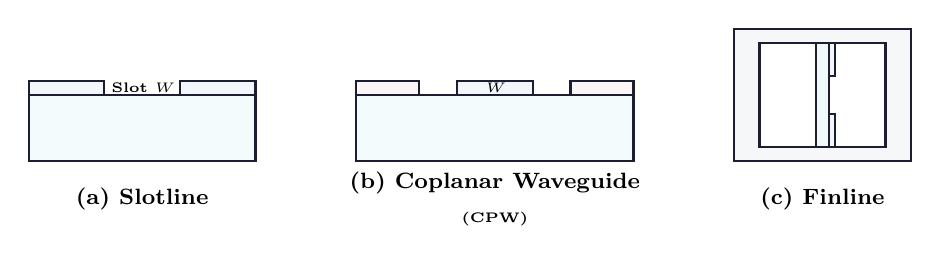
\begin{tikzpicture}[x=1.6cm, y=1.2cm]
  % Slotline
  \draw[line, fill=hdrteal!30] (0,0) rectangle (1.8,0.7);
  \draw[line, fill=hdrblue!60] (0,0.7) rectangle (0.6,0.85); % Left metal
  \draw[line, fill=hdrblue!60] (1.2,0.7) rectangle (1.8,0.85); % Right metal
  \node at (0.9,0.775) {\tiny\textbf{Slot $W$}};
  \node[align=center] at (0.9,-0.4) {\footnotesize\textbf{(a) Slotline}};
  
  % CPW
  \draw[line, fill=hdrteal!30] (2.6,0) rectangle (4.8,0.7);
  \draw[line, fill=hdrred!40] (2.6,0.7) rectangle (3.1,0.85); % Ground 1
  \draw[line, fill=hdrblue!60] (3.4,0.7) rectangle (4.0,0.85); % Center Strip
  \draw[line, fill=hdrred!40] (4.3,0.7) rectangle (4.8,0.85); % Ground 2
  \node at (3.7,0.775) {\tiny\textbf{$W$}};
  \node[align=center] at (3.7,-0.4) {\footnotesize\textbf{(b) Coplanar Waveguide}\\\tiny\textbf{(CPW)}};
  
  % Finline
  \draw[line, fill=mygray] (5.6,0) rectangle (7.0,1.4); % Waveguide box
  \draw[line, fill=white] (5.8,0.15) rectangle (6.8,1.25); % Inner cavity
  \draw[line, fill=hdrteal!40] (6.25,0.15) rectangle (6.35,1.25); % E-plane Substrate
  \draw[line, fill=hdrblue!60] (6.35,0.15) rectangle (6.4,0.5); % Bottom Fin
  \draw[line, fill=hdrblue!60] (6.35,0.9) rectangle (6.4,1.25); % Top Fin
  \node[align=center] at (6.3,-0.4) {\footnotesize\textbf{(c) Finline}};
\end{tikzpicture}
\end{tcolorbox}

\begin{tcolorbox}[examplebox, title={Worked Numerical: Coplanar Waveguide Impedance Calculation}]
  \textbf{Problem:} A Coplanar Waveguide (CPW) is fabricated on a GaAs substrate ($\varepsilon_r = 12.9$). Calculate:
  \begin{enumerate}[label=(\alph*), noitemsep]
    \item The effective dielectric constant $\varepsilon_{eff,CPW}$.
    \item The characteristic impedance $Z_0$ if ratio $K'(k)/K(k) = 1.0$.
  \end{enumerate}
  \tcblower
  \textbf{Solution:}
  \begin{enumerate}[label=(\alph*), itemsep=4pt]
    \item Effective dielectric constant for symmetrical CPW:
      \begin{equation}
        \varepsilon_{eff,CPW} = \frac{\varepsilon_r + 1}{2} = \frac{12.9 + 1}{2} = 6.95
      \end{equation}
    \item Characteristic impedance calculation:
      \begin{equation}
        Z_{0,CPW} = \frac{30\pi}{\sqrt{6.95}} \times (1.0) = \frac{94.2477}{2.63628} = 35.75\text{ }\Omega
      \end{equation}
  \end{enumerate}
\end{tcolorbox}

% ===============================================================================
% QUICK REVISION PAGE
% ===============================================================================
\newpage
\begin{center}
  {\large\bfseries\color{myred} Quick Revision --- Module 3}\\[3pt]
  {\small\color{mydark} Planar Lines-II (Slotline, Finlines \& CPW) $|$ OE-EC804B}
\end{center}
\noindent{\color{myred}\rule{\linewidth}{1.2pt}}
\vspace{4pt}

\begin{tcolorbox}[formulabox, title={\textbf{Key Concepts and Metrics at a Glance}}]
\renewcommand{\arraystretch}{1.35}
\begin{tabularx}{\linewidth}{>{\raggedright\arraybackslash\bfseries}p{4.5cm} X}
Slotline Mode & Non-TEM / TE-like mode with longitudinal magnetic field $H_z \ne 0$. \\[4pt]
Transverse Resonance Method & Evaluates slotline \& finline parameters via admittance resonance $\sum Y_{transverse} = 0$. \\[4pt]
CPW Effective Dielectric & $\varepsilon_{eff,CPW} = \frac{\varepsilon_r+1}{2}$ \quad (Equal electric energy split in air and substrate). \\[4pt]
CPW Impedance & $Z_{0,CPW} = \frac{30\pi}{\sqrt{\varepsilon_{eff}}} \frac{K'(k)}{K(k)}$ \quad (Using complete elliptic integrals). \\[4pt]
Via-Hole Elimination & CPW and Slotline allow direct surface shunt mounting of active devices without via holes. \\
\end{tabularx}
\end{tcolorbox}

\begin{tcolorbox}[defbox, title={\textbf{One-Line Definitions}}]
  \begin{itemize}[leftmargin=*, noitemsep]
    \item \textbf{Slotline:} A planar line formed by a narrow slot in a conductive ground plane on a dielectric substrate.
    \item \textbf{Coplanar Waveguide (CPW):} A planar line with center conductor and dual ground planes on the same surface.
    \item \textbf{Finline:} An $E$-plane slotline enclosed inside a rectangular waveguide wall.
    \item \textbf{Transverse Resonance Method (TRM):} Analytical field method enforcing zero net input admittance across transverse cut planes.
  \end{itemize}
\end{tcolorbox}

\begin{tcolorbox}[exambox, title={\textbf{Frequently Asked / Viva Questions}}]
  \begin{enumerate}[topsep=0pt, label=\textbf{Q\arabic*.}, itemsep=5pt]
    \item \Q{What is the dominant propagation mode in a slotline?}
    Slotline supports a non-TEM TE-like mode with a transverse electric field $E_y$ and longitudinal magnetic field $H_z$.

    \item \Q{Compare Slotline and Microstrip line.}
    Microstrip uses a Quasi-TEM mode with $20\text{ }\Omega$--$120\text{ }\Omega$ impedance and requires via holes for shunt mounting. Slotline uses a TE-like mode with $50\text{ }\Omega$--$300\text{ }\Omega$ impedance and allows direct surface shunt mounting.

    \item \Q{Why does Coplanar Waveguide (CPW) eliminate the need for via holes?}
    Because both signal conductor and ground planes reside on the top surface of the substrate, allowing active devices to be connected directly in shunt.

    \item \Q{Explain the Transverse Resonance Method (TRM).}
    TRM models the cross-section of a non-TEM transmission line as a transverse resonant line, finding $\beta$ by setting total transverse input admittance $\sum Y(y) = 0$.

    \item \Q{What is a Finline? Name its three main structural variations.}
    A Finline is an $E$-plane slotline enclosed inside a metallic rectangular waveguide. Variations: Unilateral, Bilateral, and Insulated Finlines.

    \item \Q{Why is slotline suitable for mounting non-reciprocal ferrite isolators?}
    Because the slotline magnetic field exhibits circular/elliptical polarization in the substrate region, ideal for ferrite interaction.

    \item \Q{How does the characteristic impedance of a CPW depend on gap width $S$?}
    Increasing gap width $S$ decreases total line capacitance, thereby increasing characteristic impedance $Z_0$.

    \item \Q{What is an air-bridge in CPW circuits?}
    A raised metal wire bridge connecting the dual ground planes of CPW to suppress unwanted odd-mode (slotline mode) propagation.

    \item \Q{What are the advantages of Finlines at millimeter-wave frequencies ($>30\text{ GHz}$)?}
    Combines the low loss and high power handling of rectangular waveguides with the planar circuit integration of slotlines.

    \item \Q{How does conductor loss $\alpha_c$ in Finlines vary with slot width $W$?}
    Conductor loss increases inversely with slot width ($1/W$) due to high current density concentration at fin edges.
  \end{enumerate}
\end{tcolorbox}


% -- Module 4 -----------------------------------------------------------------
\modulestart{4}{Parallel-Coupled Microstrip Lines}

\section{Parallel-Coupled Microstrip Lines}

Coupled microstrip lines consist of two unshielded, parallel microstrip conductors of width $W$ separated by a gap distance $S$ on a dielectric substrate of thickness $h$. When electromagnetic signals travel on one line, energy is coupled to the adjacent line via fringing electric and magnetic fields.

\subsection{Even-Mode and Odd-Mode Analysis}
Any arbitrary voltage and current excitation on two symmetrical coupled lines can be decomposed into two fundamental orthogonal modes:

\begin{enumerate}[leftmargin=*, itemsep=5pt]
  \item \textbf{Even Mode ($+ +$):} Both conductors are excited with equal amplitude and equal phase ($V_1 = V_2 = V_e, I_1 = I_2 = I_e$). No net current flows across the central plane of symmetry. The symmetry plane acts as an \textbf{ideal magnetic wall ($\partial E/\partial n = 0, H_{tan} = 0$)}.
  \item \textbf{Odd Mode ($+ -$):} Conductors are excited with equal amplitude but opposite phase ($V_1 = -V_2 = V_o, I_1 = -I_2 = I_o$). The zero-voltage plane of symmetry acts as an \textbf{ideal electric wall ($E_{tan} = 0$)}.
\end{enumerate}

\subsection{Characteristic Impedances (\texorpdfstring{$Z_{0e}, Z_{0o}$}{Z0e, Z0o}) \& Coupling Equations}

\begin{tcolorbox}[formulabox, title={Coupled Line Impedance \& Coupling Formulas}]
  The system characteristic impedance $Z_0$ and voltage coupling coefficient $C$ are uniquely determined by even-mode impedance $Z_{0e}$ and odd-mode impedance $Z_{0o}$:
  \begin{equation}
    Z_0 = \sqrt{Z_{0e} \cdot Z_{0o}} \quad ; \quad C = \frac{Z_{0e} - Z_{0o}}{Z_{0e} + Z_{0o}}
  \end{equation}
  Inverting these relations yields design formulas for $Z_{0e}$ and $Z_{0o}$ given $Z_0$ and coupling factor $C$:
  \begin{equation}
    Z_{0e} = Z_0 \sqrt{\frac{1+C}{1-C}} \quad ; \quad Z_{0o} = Z_0 \sqrt{\frac{1-C}{1+C}}
  \end{equation}
\end{tcolorbox}

\subsection{Quarter-Wave Coupling Region Length}
For a single-section coupled line directional coupler, maximum power coupling occurs when the physical length $L$ of the coupled region is a quarter guided wavelength ($\lambda_g/4$):
\begin{equation}
  L = \frac{\lambda_g}{4} = \frac{c}{4 f \sqrt{\varepsilon_{eff,avg}}} \quad \text{where } \varepsilon_{eff,avg} \approx \frac{\varepsilon_{eff,e} + \varepsilon_{eff,o}}{2}
\end{equation}

\begin{tcolorbox}[examplebox, title={Worked Numerical: $10\text{ dB}$ Coupled Line Design}]
  \textbf{Problem:} Design a $10\text{ dB}$ microstrip directional coupler in a $50\text{ }\Omega$ system. Calculate the required even-mode ($Z_{0e}$) and odd-mode ($Z_{0o}$) characteristic impedances.
  \tcblower
  \textbf{Solution:}
  \begin{enumerate}[label=Step \arabic*:, itemsep=4pt]
    \item Convert coupling factor $C_{\text{dB}} = 10\text{ dB}$ to voltage coupling ratio $C$:
      \begin{equation}
        \begin{aligned}
          C_{\text{dB}} &= 20 \log_{10}\left(\frac{1}{C}\right) = 10 \implies \log_{10}(C) = -0.5 \\
          &\implies C = 10^{-0.5} = 0.3162
        \end{aligned}
      \end{equation}
    \item Calculate $Z_{0e}$ and $Z_{0o}$ for $Z_0 = 50\text{ }\Omega$:
      \begin{equation}
        \begin{aligned}
          Z_{0e} &= 50 \sqrt{\frac{1 + 0.3162}{1 - 0.3162}} = 50 \sqrt{\frac{1.3162}{0.6838}} \\
          &= 50 \sqrt{1.9248} = 50 \times 1.3874 = 69.37\text{ }\Omega
        \end{aligned}
      \end{equation}
      \begin{equation}
        Z_{0o} = 50 \sqrt{\frac{1 - 0.3162}{1 + 0.3162}} = 50 \sqrt{0.5195} = 50 \times 0.7208 = 36.04\text{ }\Omega
      \end{equation}
    \item Check consistency: $Z_0 = \sqrt{Z_{0e} Z_{0o}} = \sqrt{69.37 \times 36.04} = \sqrt{2500} = 50.0\text{ }\Omega$ (Correct!).
  \end{enumerate}
\end{tcolorbox}

% ===============================================================================
% 2. BRANCH-LINE COUPLER AND RAT-RACE HYBRID RING
% ===============================================================================
\section{Branch-Line Coupler and Rat-Race Hybrid Ring}

\subsection{Branch-Line Power Divider ($3\text{ dB}$, $90^\circ$ Quadrature Hybrid)}
A \textbf{Branch-Line Coupler} is a 4-port symmetrical directional coupler consisting of four $\lambda_g/4$ microstrip arms forming a rectangular ring.

\begin{tcolorbox}[masonbox, title={Branch-Line Coupler Design Parameters}]
  For a $3\text{ dB}$ equal power split in a $50\text{ }\Omega$ system ($Z_0 = 50\text{ }\Omega$):
  \begin{itemize}[leftmargin=*, noitemsep]
    \item Horizontal main series arms impedance: $Z_A = \frac{Z_0}{\sqrt{2}} = \frac{50}{\sqrt{2}} \approx 35.35\text{ }\Omega$.
    \item Vertical shunt branch arms impedance: $Z_B = Z_0 = 50\text{ }\Omega$.
    \item All 4 branch lengths are exactly $L = \lambda_g/4$.
  \end{itemize}
\end{tcolorbox}

\subsubsection{Scattering Matrix ($[S]$) of Branch-Line Coupler}
When signal is fed at Port 1, power splits equally between Port 2 ($0^\circ$) and Port 3 ($-90^\circ$), while Port 4 is fully isolated ($S_{41} = 0$):
\begin{equation}
  [S]_{\text{Branch-Line}} = -\frac{1}{\sqrt{2}} \begin{bmatrix} 0 & j & 1 & 0 \\ j & 0 & 0 & 1 \\ 1 & 0 & 0 & j \\ 0 & 1 & j & 0 \end{bmatrix}
\end{equation}

\subsection{Rat-Race Hybrid Ring ($180^\circ$ Hybrid)}
A \textbf{Rat-Race Coupler} consists of a circular microstrip ring of total perimeter $1.5\lambda_g$ ($6\theta = 540^\circ$) with 4 ports. Ports 1, 2, 3, and 4 are separated by $\lambda_g/4$ gaps, except between Port 3 and Port 4 which are separated by a $3\lambda_g/4$ gap.

\begin{tcolorbox}[formulabox, title={Rat-Race Impedance \& Scattering Matrix}]
  Ring characteristic impedance: $Z_{\text{ring}} = \sqrt{2} Z_0 \approx 70.7\text{ }\Omega$ (for $Z_0 = 50\text{ }\Omega$).
  \begin{equation}
    [S]_{\text{Rat-Race}} = -\frac{j}{\sqrt{2}} \begin{bmatrix} 0 & 1 & 0 & -1 \\ 1 & 0 & 1 & 0 \\ 0 & 1 & 0 & 1 \\ -1 & 0 & 1 & 0 \end{bmatrix}
  \end{equation}
  \begin{itemize}[leftmargin=*, noitemsep]
    \item \textbf{Sum Port ($\Sigma$ / Port 1):} Input at Port 1 splits equally in-phase ($0^\circ$) between Ports 2 and 4. Port 3 is isolated due to destructive interference ($180^\circ$ path difference).
    \item \textbf{Difference Port ($\Delta$ / Port 3):} Input at Port 3 splits equally out-of-phase ($180^\circ$) between Ports 2 and 4. Port 1 is isolated.
  \end{itemize}
\end{tcolorbox}

\begin{tcolorbox}[tikzbox, title={Topologies of Branch-Line Coupler ($90^\circ$) and Rat-Race Hybrid Ring ($180^\circ$)}]
\centering
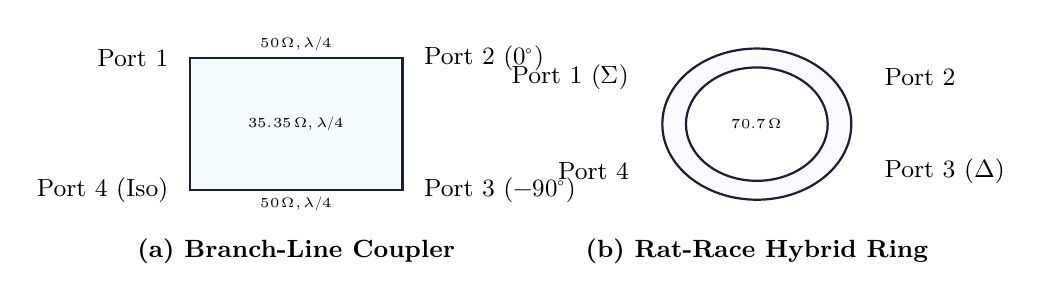
\begin{tikzpicture}[x=1.5cm, y=1.2cm]
  % Branch Line Coupler
  \draw[line, fill=hdrteal!30] (0,0) rectangle (1.8,1.4);
  \node at (0.9,0.7) {\tiny\textbf{$35.35\,\Omega, \lambda/4$}};
  \node at (0.9,1.55) {\tiny\textbf{$50\,\Omega, \lambda/4$}};
  \node at (0.9,-0.15) {\tiny\textbf{$50\,\Omega, \lambda/4$}};
  \node[anchor=east] at (-0.1,1.4) {\small Port 1};
  \node[anchor=west] at (1.9,1.4) {\small Port 2 ($0^\circ$)};
  \node[anchor=east] at (-0.1,0) {\small Port 4 (Iso)};
  \node[anchor=west] at (1.9,0) {\small Port 3 ($-90^\circ$)};
  \node[align=center] at (0.9,-0.65) {\small\textbf{(a) Branch-Line Coupler}};

  % Rat Race Hybrid Ring
  \draw[line, fill=hdrpurple!20] (4.8,0.7) circle (0.8);
  \draw[line, fill=white] (4.8,0.7) circle (0.6);
  \node at (4.8,0.7) {\tiny\textbf{$70.7\,\Omega$}};
  \node[anchor=east] at (3.8,1.2) {\small Port 1 ($\Sigma$)};
  \node[anchor=west] at (5.8,1.2) {\small Port 2};
  \node[anchor=west] at (5.8,0.2) {\small Port 3 ($\Delta$)};
  \node[anchor=east] at (3.8,0.2) {\small Port 4};
  \node[align=center] at (4.8,-0.65) {\small\textbf{(b) Rat-Race Hybrid Ring}};
\end{tikzpicture}
\end{tcolorbox}

% ===============================================================================
% QUICK REVISION PAGE
% ===============================================================================
\newpage
\begin{center}
  {\large\bfseries\color{myred} Quick Revision --- Module 4}\\[3pt]
  {\small\color{mydark} Parallel-Coupled Microstrip Lines \& Power Dividers $|$ OE-EC804B}
\end{center}
\noindent{\color{myred}\rule{\linewidth}{1.2pt}}
\vspace{4pt}

\begin{tcolorbox}[formulabox, title={\textbf{Key Concepts and Metrics at a Glance}}]
\renewcommand{\arraystretch}{1.35}
\begin{tabularx}{\linewidth}{>{\raggedright\arraybackslash\bfseries}p{4.5cm} X}
System Impedance $Z_0$ & $Z_0 = \sqrt{Z_{0e} \cdot Z_{0o}}$ \quad (Geometric mean of even and odd mode impedances) \\[4pt]
Voltage Coupling Factor $C$ & $C = \frac{Z_{0e} - Z_{0o}}{Z_{0e} + Z_{0o}} \implies Z_{0e} = Z_0 \sqrt{\frac{1+C}{1-C}}, Z_{0o} = Z_0 \sqrt{\frac{1-C}{1+C}}$. \\[4pt]
Branch-Line Arm Impedances & Main series arms $Z_A = Z_0 / \sqrt{2} = 35.35\text{ }\Omega$; Branch arms $Z_B = Z_0 = 50\text{ }\Omega$. \\[4pt]
Rat-Race Ring Impedance & Ring characteristic impedance $Z_{\text{ring}} = \sqrt{2} Z_0 = 70.7\text{ }\Omega$. \\[4pt]
Rat-Race Arm Spacings & 3 sections of $\lambda_g/4$ and 1 section of $3\lambda_g/4$ (Total perimeter $1.5\lambda_g$). \\
\end{tabularx}
\end{tcolorbox}

\begin{tcolorbox}[defbox, title={\textbf{One-Line Definitions}}]
  \begin{itemize}[leftmargin=*, noitemsep]
    \item \textbf{Even Mode ($Z_{0e}$):} Symmetrical mode where coupled line currents flow in identical directions with magnetic wall symmetry.
    \item \textbf{Odd Mode ($Z_{0o}$):} Anti-symmetrical mode where coupled line currents flow in opposite directions with electric wall symmetry.
    \item \textbf{Quadrature Hybrid ($90^\circ$):} Directional coupler providing equal power division with $90^\circ$ phase shift between output ports.
    \item \textbf{Rat-Race Ring ($180^\circ$):} 4-port hybrid ring providing equal in-phase ($0^\circ$) or anti-phase ($180^\circ$) power division.
  \end{itemize}
\end{tcolorbox}

\begin{tcolorbox}[exambox, title={\textbf{Frequently Asked / Viva Questions}}]
  \begin{enumerate}[topsep=0pt, label=\textbf{Q\arabic*.}, itemsep=5pt]
    \item \Q{Define even-mode and odd-mode impedances ($Z_{0e}, Z_{0o}$) of coupled microstrip lines.}
    $Z_{0e}$ is the characteristic impedance when lines are driven in-phase with equal currents. $Z_{0o}$ is the impedance when lines are driven out-of-phase with opposite currents.

    \item \Q{How is characteristic impedance $Z_0$ related to $Z_{0e}$ and $Z_{0o}$?}
    $Z_0 = \sqrt{Z_{0e} \cdot Z_{0o}}$.

    \item \Q{What is the physical length of a parallel-coupled microstrip directional coupler?}
    The coupled region length $L = \lambda_g/4$ at the center frequency.

    \item \Q{Explain the operation of a $3\text{ dB}$ Branch-Line Coupler.}
    A 4-port quadrature hybrid consisting of four $\lambda_g/4$ branches. Input at Port 1 splits equally between Port 2 ($0^\circ$) and Port 3 ($-90^\circ$), with Port 4 isolated.

    \item \Q{What are the arm impedances of a $50\text{ }\Omega$ Branch-Line Coupler?}
    The horizontal series arms have impedance $Z_0/\sqrt{2} = 35.35\text{ }\Omega$, and vertical shunt branch arms have impedance $Z_0 = 50\text{ }\Omega$.

    \item \Q{Describe the structure and port spacing of a Rat-Race Hybrid Ring.}
    A circular ring of characteristic impedance $\sqrt{2}Z_0 = 70.7\text{ }\Omega$ with 4 ports. Three port gaps are $\lambda_g/4$ and one gap is $3\lambda_g/4$ (total perimeter $1.5\lambda_g$).

    \item \Q{How does the Rat-Race coupler operate as a sum ($\Sigma$) and difference ($\Delta$) network?}
    Input at Port 1 splits in-phase ($0^\circ$) at Ports 2 and 4 ($\Sigma$ mode). Input at Port 3 splits out-of-phase ($180^\circ$) at Ports 2 and 4 ($\Delta$ mode).

    \item \Q{What causes directivity degradation in microstrip coupled lines?}
    Phase velocity mismatch between even mode ($\beta_e$) and odd mode ($\beta_o$), caused by non-homogeneous substrate/air dielectric boundary.

    \item \Q{How is crosstalk defined in parallel-coupled lines?}
    Crosstalk is unwanted electromagnetic power coupling from a driven primary line to an adjacent secondary signal line.

    \item \Q{What is the bandwidth restriction of branch-line and rat-race couplers?}
    They are narrowband components ($\approx 10\% - 20\%$ bandwidth) because their operation relies on exact $\lambda_g/4$ line lengths.
  \end{enumerate}
\end{tcolorbox}


% -- Module 5 -----------------------------------------------------------------
\modulestart{5}{MIC Measurement Systems, Fixtures and Probes}

\section{MIC Measurement Systems, Fixtures and Probes}

Testing unpackaged MIC/MMIC chips presents unique challenges because standard coaxial cables (SMA, $2.92\text{ mm}$, $1.85\text{ mm}$) cannot interface directly with sub-millimeter planar microstrip pads on semiconductor wafers.

\begin{tcolorbox}[defbox, title={Microwave Test Fixture \& On-Wafer Probes}]
  A \textbf{Microwave Test Fixture} holds packaged or unpackaged MIC substrates and provides low-reflection transitions from coaxial launchers to planar microstrip traces. \textbf{On-Wafer RF Probes} (Ground-Signal-Ground / GSG coplanar probes) make direct electrical contact with MMIC pads on the semiconductor wafer using precision micro-positioning manipulators, operating up to $110\text{ GHz}$.
\end{tcolorbox}

\subsection{Wafer Probe Architecture (GSG Configuration)}
Coplanar GSG probes maintain a continuous $50\text{ }\Omega$ coplanar transmission line right up to the beryllium-copper or tungsten probe tips, completely eliminating wire bond series inductance ($L_s \approx 0$) during wafer-level characterization.

% ===============================================================================
% 2. S-PARAMETER MEASUREMENT AND CALIBRATION
% ===============================================================================
\section{S-Parameter Measurement and Calibration}

\subsection{Vector Network Analyzer (VNA)}
A \textbf{Vector Network Analyzer (VNA)} measures both the magnitude and phase of 2-port scattering parameters ($S_{11}, S_{21}, S_{12}, S_{22}$) by transmitting a frequency-swept RF signal and separating incident, reflected, and transmitted waves using internal directional couplers and heterodyne receivers.

\subsection{VNA Calibration \& Systematic De-Embedding}
Uncalibrated VNA measurements include systematic errors caused by cable attenuation, connector reflections, directional coupler directivity limits, and receiver frequency response. Calibration establishes mathematical error models to de-embed the fixture and move the measurement reference plane to the device under test (DUT).

\begin{enumerate}[leftmargin=*, itemsep=5pt]
  \item \textbf{SOLT Calibration (Short-Open-Load-Thru):}
    \begin{itemize}[leftmargin=*, noitemsep]
      \item Standard calibration for coaxial measurements using 4 known standards: Short ($\Gamma = -1$), Open ($\Gamma = +1$), Matched Load ($\Gamma = 0$), and Thru line ($S_{21} = 1$).
      \item \textit{Limitation in MMIC Testing:} Fabricating a precise, broadband $50\text{ }\Omega$ matched load standard on a semiconductor substrate is extremely difficult due to parasitic capacitance.
    \end{itemize}
  \item \textbf{TRL Calibration (Thru-Reflect-Line):}
    \begin{itemize}[leftmargin=*, noitemsep]
      \item Uses 3 simple planar standards printed directly on the substrate: a \textbf{Thru} line ($0$ length), an unknown high-reflection \textbf{Reflect} standard (Short or Open with identical $|\Gamma| \approx 1$), and a \textbf{Line} standard ($\lambda_g/4$ longer than Thru).
      \item \textbf{Primary calibration method for MMIC wafer probing} because it does not require a $50\text{ }\Omega$ matched load standard.
    \end{itemize}
\end{enumerate}

\begin{tcolorbox}[tikzbox, title={Vector Network Analyzer (VNA) S-Parameter Measurement Setup}]
\centering

\begin{tikzpicture}[
  node distance=0.5cm, auto,
  sblock/.style={draw=myteal, fill=hdrteal, rectangle, rounded corners=3pt, align=center, font=\small\bfseries, minimum height=0.9cm, text width=2.3cm}
]
  \node [sblock] (vna) {Vector Network\\Analyzer (VNA)};
  \node [sblock, right=0.5cm of vna] (coupler) {Dual Directional\\Couplers};
  \node [sblock, fill=hdrpurple!30, draw=mypurple, right=0.5cm of coupler] (probe) {GSG Probe /\\Test Fixture};
  \node [sblock, fill=hdrred!30, draw=myred, right=0.5cm of probe] (dut) {MIC / MMIC\\Device Under Test};

  \draw [arrow] (vna) -- (coupler);
  \draw [arrow] (coupler) -- (probe);
  \draw [arrow] (probe) -- (dut);
\end{tikzpicture}
\end{tcolorbox}

% ===============================================================================
% 3. NOISE MEASUREMENT TECHNIQUES
% ===============================================================================
\section{Noise Figure Measurement Techniques}

Noise Figure ($NF$) measures the degradation of Signal-to-Noise Ratio (SNR) as a signal passes through a microwave circuit:
\begin{equation}
  F = \frac{\text{SNR}_{in}}{\text{SNR}_{out}} \quad ; \quad NF (\text{dB}) = 10 \log_{10}(F)
\end{equation}

\subsection{The Y-Factor Measurement Method}
The \textbf{Y-Factor Method} is the industry standard technique for measuring Noise Figure using a calibrated noise source toggled between two known noise temperatures: \textbf{HOT ($T_H$)} and \textbf{COLD ($T_C$)}.

\begin{tcolorbox}[formulabox, title={Y-Factor Derivation \& Noise Figure Equations}]
  Noise power measured at receiver output for HOT and COLD states:
  \begin{equation}
    N_{\text{HOT}} = k (T_H + T_e) B \cdot G \quad ; \quad N_{\text{COLD}} = k (T_C + T_e) B \cdot G
  \end{equation}
  Taking the ratio yields the dimensionless $Y$-factor:
  \begin{equation}
    Y = \frac{N_{\text{HOT}}}{N_{\text{COLD}}} = \frac{T_H + T_e}{T_C + T_e} \implies T_e = \frac{T_H - Y T_C}{Y - 1}
  \end{equation}
  The noise factor $F$ relative to reference temperature $T_0 = 290\text{ K}$ ($27^\circ\text{C}$):
  \begin{equation}
    F = 1 + \frac{T_e}{T_0} = \frac{\text{ENR}}{Y - 1} \quad \text{where } \text{ENR} = \frac{T_H - T_0}{T_0} \text{ (Excess Noise Ratio)}
  \end{equation}
\end{tcolorbox}

\begin{tcolorbox}[examplebox, title={Worked Numerical: Noise Figure Calculation via Y-Factor Method}]
  \textbf{Problem:} A noise source with an Excess Noise Ratio $\text{ENR} = 15.0\text{ dB}$ is connected to a microwave amplifier. The measured output noise power ratio between HOT and COLD states is $Y = 8.0\text{ dB}$. Calculate:
  \begin{enumerate}[label=(\alph*), noitemsep]
    \item The linear ENR and linear $Y$-factor.
    \item The Noise Factor $F$ and Noise Figure $NF$ in dB.
  \end{enumerate}
  \tcblower
  \textbf{Solution:}
  \begin{enumerate}[label=(\alph*), itemsep=4pt]
    \item Convert values from dB to linear ratios:
      \begin{equation}
        \text{ENR}_{\text{linear}} = 10^{15/10} = 10^{1.5} = 31.6228
      \end{equation}
      \begin{equation}
        Y_{\text{linear}} = 10^{8/10} = 10^{0.8} = 6.30957
      \end{equation}
    \item Calculate Noise Factor $F$:
      \begin{equation}
        \begin{aligned}
          F &= \frac{\text{ENR}_{\text{linear}}}{Y_{\text{linear}} - 1} = \frac{31.6228}{6.30957 - 1} \\
          &= \frac{31.6228}{5.30957} = 5.9558
        \end{aligned}
      \end{equation}
      Convert $F$ to Noise Figure $NF$ in dB:
      \begin{equation}
        NF = 10 \log_{10}(5.9558) = 7.749\text{ dB} \approx 7.75\text{ dB}
      \end{equation}
  \end{enumerate}
\end{tcolorbox}

% ===============================================================================
% QUICK REVISION PAGE
% ===============================================================================
\newpage
\begin{center}
  {\large\bfseries\color{myred} Quick Revision --- Module 5}\\[3pt]
  {\small\color{mydark} MIC Measurement, Testing \& Applications $|$ OE-EC804B}
\end{center}
\noindent{\color{myred}\rule{\linewidth}{1.2pt}}
\vspace{4pt}

\begin{tcolorbox}[formulabox, title={\textbf{Key Concepts and Metrics at a Glance}}]
\renewcommand{\arraystretch}{1.35}
\begin{tabularx}{\linewidth}{>{\raggedright\arraybackslash\bfseries}p{4.5cm} X}
Vector Network Analyzer (VNA) & Measures magnitude \& phase of 2-port S-parameters ($S_{11}, S_{21}, S_{12}, S_{22}$). \\[4pt]
TRL Calibration & Thru-Reflect-Line method; preferred for MMIC wafer probes as no matched load standard is required. \\[4pt]
GSG Wafer Probes & Ground-Signal-Ground coplanar probes providing $50\text{ }\Omega$ contact directly to MMIC pads. \\[4pt]
Y-Factor Noise Measurement & Toggles noise source between HOT ($T_H$) and COLD ($T_C$) states ($Y = N_{\text{HOT}}/N_{\text{COLD}}$). \\[4pt]
Excess Noise Ratio (ENR) & $\text{ENR} = (T_H - T_0)/T_0$; specifies calibrated output power of RF noise head. \\
\end{tabularx}
\end{tcolorbox}

\begin{tcolorbox}[defbox, title={\textbf{One-Line Definitions}}]
  \begin{itemize}[leftmargin=*, noitemsep]
    \item \textbf{VNA:} Microwave instrument measuring complex reflection and transmission parameters of RF networks.
    \item \textbf{GSG Probe:} High-frequency coplanar probe contacting MMIC wafer pads without wire bond inductance.
    \item \textbf{TRL Calibration:} De-embedding calibration technique utilizing Thru, Reflect, and Line standards on substrate.
    \item \textbf{Y-Factor Method:} Standard microwave technique for measuring Noise Figure via hot/cold noise ratio.
  \end{itemize}
\end{tcolorbox}

\begin{tcolorbox}[exambox, title={\textbf{Frequently Asked / Viva Questions}}]
  \begin{enumerate}[topsep=0pt, label=\textbf{Q\arabic*.}, itemsep=5pt]
    \item \Q{What is the function of a Vector Network Analyzer (VNA)?}
    A VNA measures the complex scattering parameters ($S$-parameters: magnitude and phase) of microwave components over a swept frequency range.

    \item \Q{Why is calibration required before performing VNA measurements?}
    Calibration removes systematic errors introduced by test cables, connectors, attenuators, and internal VNA directional couplers.

    \item \Q{Differentiate between SOLT and TRL calibration.}
    SOLT uses Short, Open, Load, and Thru coaxial standards. TRL uses Thru, Reflect, and Line planar standards and is preferred for MMIC on-wafer probing because it does not require a $50\text{ }\Omega$ matched load standard.

    \item \Q{What is an On-Wafer GSG Probe?}
    A Ground-Signal-Ground coplanar RF probe that makes direct electrical contact with MMIC pads on the semiconductor wafer up to $110\text{ GHz}$.

    \item \Q{Explain the Y-Factor method for Noise Figure measurement.}
    The Y-Factor method measures output noise power when a noise source is switched HOT ($T_H$) and COLD ($T_C$). The ratio $Y = N_{\text{HOT}}/N_{\text{COLD}}$ determines effective noise temperature $T_e$ and Noise Figure $NF$.

    \item \Q{Define Excess Noise Ratio (ENR) of a noise source.}
    $\text{ENR} = (T_H - T_0)/T_0$, expressed in dB. It quantifies the calibrated noise power output above standard room temperature ($T_0 = 290\text{ K}$).

    \item \Q{What is a microwave test fixture?}
    A mechanical housing that holds an unencapsulated MIC substrate and provides low-reflection transitions between coaxial cables and planar microstrip lines.

    \item \Q{What is reference plane shift in S-parameter measurements?}
    The mathematical offset applied by VNA calibration to move the measurement plane from the coaxial cable tips directly to the MIC substrate ports.

    \item \Q{Why is Noise Figure measurement sensitive to receiver gain?}
    High receiver gain prevents internal meter noise from masking the small noise power differences ($N_{\text{HOT}} - N_{\text{COLD}}$) generated by the Device Under Test.

    \item \Q{What is the role of de-embedding in MIC testing?}
    De-embedding mathematically subtracts the known parasitic $S$-parameters of test fixtures and launches from the measured data to isolate the intrinsic MIC device response.
  \end{enumerate}
\end{tcolorbox}


\end{document}
